% Make the following changes to mushroomhunter.nlogo
%
% 1) There is only one hunter instead of two
% 2) Instead of 4 mushroom clusters that each have 20 mushrooms, have 8 clusters
%       with 10 mushrooms per cluster. Increase the radius to only 3 patches.
% 3) If the hunter has not recently found a mushroom, it turn by a random angle
%       between -45 and 45 degrees
\documentclass{hw}

\usepackage{minted}

\begin{document}
\makeheader{on NetLogo}

\begin{enumerate}
\item Modeling with only one hunter rather than two.

\begin{minipage}{0.5\textwidth}
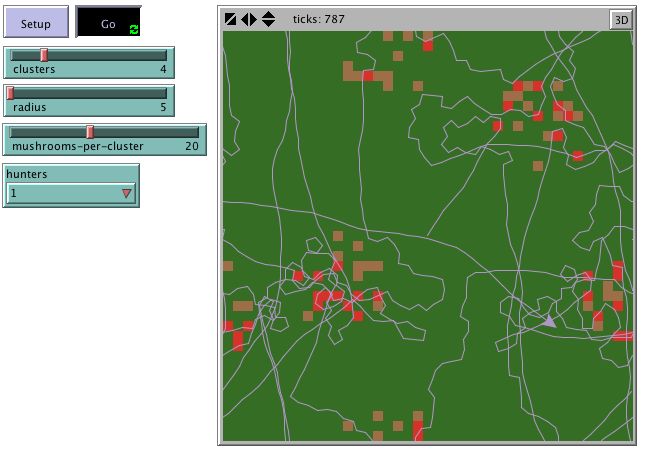
\includegraphics[scale=0.35]{one_hunter.png}
\end{minipage}
\begin{minipage}{0.5\textwidth}
\begin{minted}{lisp}
;; Setup the mushroom hunters
;; hunters is a global variable determined by the
;; chooser
  crt hunters [
    set size 2
    set color violet + 2
    set time-since-last-found 999
    pen-down
  ]
\end{minted}
\end{minipage}

\item Instead of 4 mushroom clusters that each have 20 mushrooms, have 8 clusters with 10 mushrooms per
cluster. Increase the radius to only 3 patches.

\begin{minipage}{0.5\textwidth}
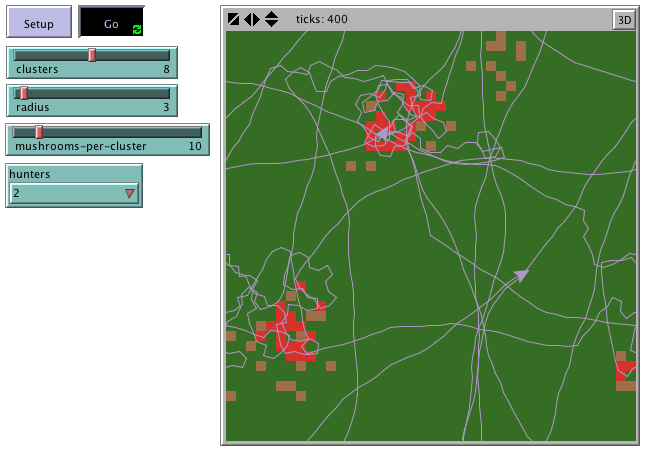
\includegraphics[scale=0.35]{more_clusters.png}
\end{minipage}
\begin{minipage}{0.5\textwidth}
\begin{minted}{lisp}
;; mushrooms-per-cluster is a global determined
;; by the slider.
;;
;; radius is a global determined by a slider
ask n-of mushrooms-per-cluster
patches in-radius radius [
  set pcolor brown
]
\end{minted}
\end{minipage}

\item If the hunter has not recently found a mushroom, it turn by a random angle
between -45 and 45 degrees.

\begin{minipage}{0.3\textwidth}
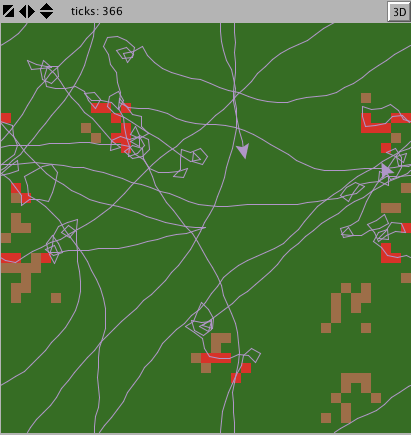
\includegraphics[scale=0.3]{ff_01.png}
\end{minipage}
\begin{minipage}{0.3\textwidth}
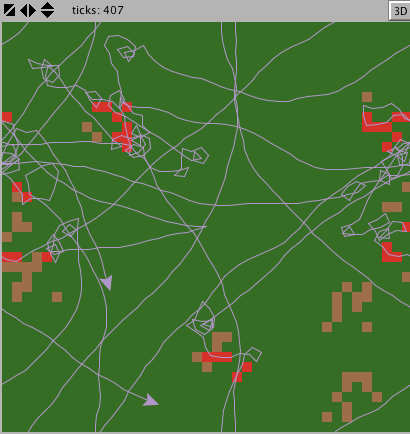
\includegraphics[scale=0.3]{ff_02.png}
\end{minipage}
\begin{minipage}{0.3\textwidth}
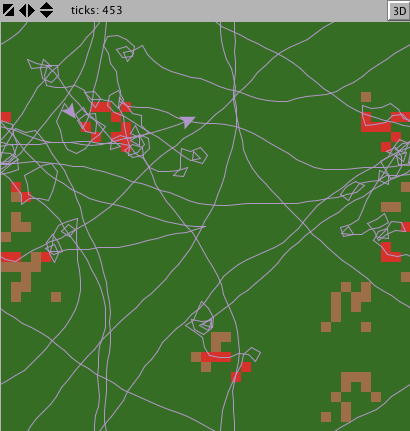
\includegraphics[scale=0.3]{ff_03.png}
\end{minipage}

\begin{minted}{lisp}
ifelse time-since-last-found <= 20
[right (random 181) - 45]
[right (random 21) - 10]
\end{minted}

\end{enumerate}
\end{document}
